\documentclass[twoside]{book}

% Packages required by doxygen
\usepackage{fixltx2e}
\usepackage{calc}
\usepackage{doxygen}
\usepackage{graphicx}
\usepackage[utf8]{inputenc}
\usepackage{makeidx}
\usepackage{multicol}
\usepackage{multirow}
\PassOptionsToPackage{warn}{textcomp}
\usepackage{textcomp}
\usepackage[nointegrals]{wasysym}
\usepackage[table]{xcolor}

% Font selection
\usepackage[T1]{fontenc}
\usepackage{mathptmx}
\usepackage[scaled=.90]{helvet}
\usepackage{courier}
\usepackage{amssymb}
\usepackage{sectsty}
\renewcommand{\familydefault}{\sfdefault}
\allsectionsfont{%
  \fontseries{bc}\selectfont%
  \color{darkgray}%
}
\renewcommand{\DoxyLabelFont}{%
  \fontseries{bc}\selectfont%
  \color{darkgray}%
}
\newcommand{\+}{\discretionary{\mbox{\scriptsize$\hookleftarrow$}}{}{}}

% Page & text layout
\usepackage{geometry}
\geometry{%
  a4paper,%
  top=2.5cm,%
  bottom=2.5cm,%
  left=2.5cm,%
  right=2.5cm%
}
\tolerance=750
\hfuzz=15pt
\hbadness=750
\setlength{\emergencystretch}{15pt}
\setlength{\parindent}{0cm}
\setlength{\parskip}{0.2cm}
\makeatletter
\renewcommand{\paragraph}{%
  \@startsection{paragraph}{4}{0ex}{-1.0ex}{1.0ex}{%
    \normalfont\normalsize\bfseries\SS@parafont%
  }%
}
\renewcommand{\subparagraph}{%
  \@startsection{subparagraph}{5}{0ex}{-1.0ex}{1.0ex}{%
    \normalfont\normalsize\bfseries\SS@subparafont%
  }%
}
\makeatother

% Headers & footers
\usepackage{fancyhdr}
\pagestyle{fancyplain}
\fancyhead[LE]{\fancyplain{}{\bfseries\thepage}}
\fancyhead[CE]{\fancyplain{}{}}
\fancyhead[RE]{\fancyplain{}{\bfseries\leftmark}}
\fancyhead[LO]{\fancyplain{}{\bfseries\rightmark}}
\fancyhead[CO]{\fancyplain{}{}}
\fancyhead[RO]{\fancyplain{}{\bfseries\thepage}}
\fancyfoot[LE]{\fancyplain{}{}}
\fancyfoot[CE]{\fancyplain{}{}}
\fancyfoot[RE]{\fancyplain{}{\bfseries\scriptsize Generated on Mon Oct 1 2018 14\+:27\+:24 for Generic Makefile by Doxygen }}
\fancyfoot[LO]{\fancyplain{}{\bfseries\scriptsize Generated on Mon Oct 1 2018 14\+:27\+:24 for Generic Makefile by Doxygen }}
\fancyfoot[CO]{\fancyplain{}{}}
\fancyfoot[RO]{\fancyplain{}{}}
\renewcommand{\footrulewidth}{0.4pt}
\renewcommand{\chaptermark}[1]{%
  \markboth{#1}{}%
}
\renewcommand{\sectionmark}[1]{%
  \markright{\thesection\ #1}%
}

% Indices & bibliography
\usepackage{natbib}
\usepackage[titles]{tocloft}
\setcounter{tocdepth}{3}
\setcounter{secnumdepth}{5}
\makeindex

% Hyperlinks (required, but should be loaded last)
\usepackage{ifpdf}
\ifpdf
  \usepackage[pdftex,pagebackref=true]{hyperref}
\else
  \usepackage[ps2pdf,pagebackref=true]{hyperref}
\fi
\hypersetup{%
  colorlinks=true,%
  linkcolor=blue,%
  citecolor=blue,%
  unicode%
}

% Custom commands
\newcommand{\clearemptydoublepage}{%
  \newpage{\pagestyle{empty}\cleardoublepage}%
}


%===== C O N T E N T S =====

\begin{document}

% Titlepage & ToC
\hypersetup{pageanchor=false,
             bookmarks=true,
             bookmarksnumbered=true,
             pdfencoding=unicode
            }
\pagenumbering{roman}
\begin{titlepage}
\vspace*{7cm}
\begin{center}%
{\Large Generic Makefile \\[1ex]\large v1.\+0.\+0 }\\
\vspace*{1cm}
{\large Generated by Doxygen 1.8.8}\\
\vspace*{0.5cm}
{\small Mon Oct 1 2018 14:27:24}\\
\end{center}
\end{titlepage}
\clearemptydoublepage
\tableofcontents
\clearemptydoublepage
\pagenumbering{arabic}
\hypersetup{pageanchor=true}

%--- Begin generated contents ---
\chapter{Generic Makefile}
\label{index}\hypertarget{index}{}\hypertarget{index_intro_sec}{}\section{Introduction}\label{index_intro_sec}
This Makefile compiles the C / C ++ sources of a project that respects a specific folders architecture. It adapts according to the binary to be generated through the different variables available.\hypertarget{index_architecture_sec}{}\section{Folder architecture}\label{index_architecture_sec}
This architecture must match the one shown below. Only the directories used by this makefile are indicated in this diagram. 
\begin{DoxyPre}
Workspace
    │
    ├──────── Project 1
    │            ├──────── build
    │            │          │
    │            │          ├──────── Debug\_<arch>
    │            │          │
    │            │          ├──────── Release\_<arch>
    │            │          │
    │            │          └──────── Test\_<arch>
    │            │
    │            ├──────── include
    │            │
    │            ├──────── log
    │            │
    │            ├──────── package
    │            │            │
    │            │            ├──────── deb
    │            │            │
    │            │            ├──────── rpm
    │            │            │
    │            │            ├──────── tar
    │            │            │
    │            │            ├──────── ...
    │            │            │
    │            │            └──────── zip
    │            │
    │            │
    │            ├──────── src
    │            │
    │            └──────── test
    │
    │
    ├──────── Project 2
    :
    :
    │
    └──────── Project n
\end{DoxyPre}
 \hypertarget{index_dir_content}{}\subsection{Directories contents}\label{index_dir_content}

\begin{DoxyItemize}
\item Workspace (\$\+W\+O\+R\+K\+S\+P\+A\+C\+E\+\_\+\+D\+I\+R) \+: Root of workspace containing all associated projects.
\item Project x (\$\+P\+R\+O\+J\+E\+C\+T\+\_\+\+D\+I\+R) \+: Roots of projects.
\item build (\$\+B\+I\+N\+\_\+\+D\+I\+R) \+: Root directory containing the generated binaries. These binaries are sorted by build configuration and by hardware architecture type.
\item build/\$\+C\+O\+N\+F\+I\+G\+\_\+\$\+T\+A\+R\+G\+E\+T\+\_\+\+A\+R\+C\+H (\$\+O\+B\+J\+\_\+\+D\+I\+R) \+: Binary specific to the build configuration.
\item include (\$\+I\+N\+C\+\_\+\+D\+I\+R) \+: Directory for public header files to be deployed with the project binary (usually for a library project)
\item log (\$\+L\+O\+G\+\_\+\+D\+I\+R) \+: Directory intended to receive the files generated by the build and control tools.
\item package (\$\+P\+A\+C\+K\+A\+G\+E\+\_\+\+D\+I\+R) \+: Root directory of subdirectories intended to receive the delivery packages.
\item src (\$\+S\+R\+C\+\_\+\+D\+I\+R) \+: Root directory of the source files. This directory can contain sub-\/directories.
\item test (\$\+T\+E\+S\+T\+\_\+\+D\+I\+R) \+: Root directory of the unit testing source files. 
\end{DoxyItemize}
\chapter{Module Index}
\section{Modules}
Here is a list of all modules\+:\begin{DoxyCompactList}
\item \contentsline{section}{Makefile}{\pageref{group___makefile}}{}
\begin{DoxyCompactList}
\item \contentsline{section}{Project Variables}{\pageref{group___project___variables}}{}
\item \contentsline{section}{Build variables}{\pageref{group___build___variables}}{}
\item \contentsline{section}{Private\+\_\+\+Variables}{\pageref{group___private___variables}}{}
\item \contentsline{section}{Automatic variables}{\pageref{group___automatic___variables}}{}
\end{DoxyCompactList}
\end{DoxyCompactList}

\chapter{File Index}
\section{File List}
Here is a list of all documented files with brief descriptions\+:\begin{DoxyCompactList}
\item\contentsline{section}{\hyperlink{_makefile}{Makefile} \\*Generic project build file }{\pageref{_makefile}}{}
\end{DoxyCompactList}

\chapter{Module Documentation}
\hypertarget{group___makefile}{\section{Makefile}
\label{group___makefile}\index{Makefile@{Makefile}}
}
Collaboration diagram for Makefile\+:
\nopagebreak
\begin{figure}[H]
\begin{center}
\leavevmode
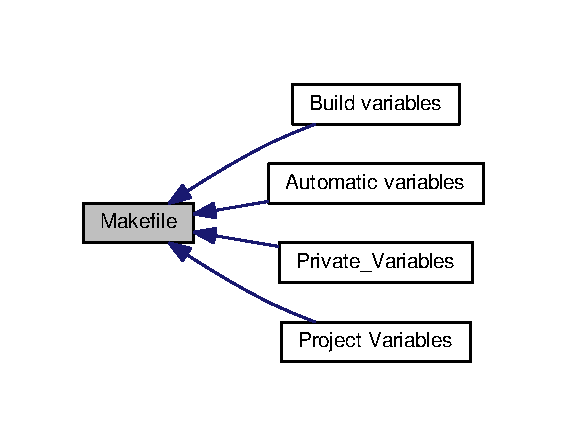
\includegraphics[width=272pt]{group___makefile}
\end{center}
\end{figure}
\subsection*{Modules}
\begin{DoxyCompactItemize}
\item 
\hyperlink{group___project___variables}{Project Variables}
\begin{DoxyCompactList}\small\item\em These variables must be declared in this file according to the project. \end{DoxyCompactList}\item 
\hyperlink{group___build___variables}{Build variables}
\begin{DoxyCompactList}\small\item\em These variables can be redefined before the execution of 'make'. \end{DoxyCompactList}\item 
\hyperlink{group___private___variables}{Private\+\_\+\+Variables}
\begin{DoxyCompactList}\small\item\em These variables. \end{DoxyCompactList}\item 
\hyperlink{group___automatic___variables}{Automatic variables}
\begin{DoxyCompactList}\small\item\em These variables can be redefined during the execution of 'make'. \end{DoxyCompactList}\end{DoxyCompactItemize}


\subsection{Detailed Description}

\hypertarget{group___project___variables}{\section{Project Variables}
\label{group___project___variables}\index{Project Variables@{Project Variables}}
}


These variables must be declared in this file according to the project.  


Collaboration diagram for Project Variables\+:
\nopagebreak
\begin{figure}[H]
\begin{center}
\leavevmode
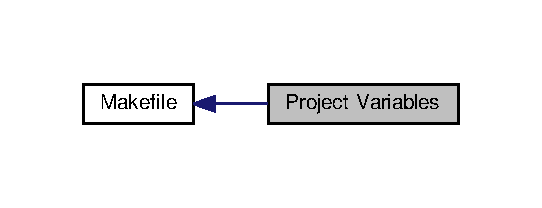
\includegraphics[width=260pt]{group___project___variables}
\end{center}
\end{figure}
\subsection*{Macros}
\begin{DoxyCompactItemize}
\item 
\hypertarget{group___project___variables_gae73053051efbb45c3a39751f5ce9fb36}{\#define \hyperlink{group___project___variables_gae73053051efbb45c3a39751f5ce9fb36}{P\+R\+O\+J\+E\+C\+T\+\_\+\+N\+A\+M\+E}}\label{group___project___variables_gae73053051efbb45c3a39751f5ce9fb36}

\begin{DoxyCompactList}\small\item\em Defines the project name. This name must match the name of the project's parent directory in the workspace. \end{DoxyCompactList}\item 
\hypertarget{group___project___variables_gad661cebbb68b497f00fba5676c36eaea}{\#define \hyperlink{group___project___variables_gad661cebbb68b497f00fba5676c36eaea}{D\+E\+P\+E\+N\+D\+E\+N\+C\+I\+E\+S}}\label{group___project___variables_gad661cebbb68b497f00fba5676c36eaea}

\begin{DoxyCompactList}\small\item\em Sets the name of libraries whose binary depends. These libraries must be in a path of the L\+D\+\_\+\+L\+I\+B\+R\+A\+R\+Y\+\_\+\+P\+A\+T\+H variable, in the system default directories, or in workspace. \end{DoxyCompactList}\item 
\hypertarget{group___project___variables_ga36eaa1244b8f912226a6211c0300afd1}{\#define \hyperlink{group___project___variables_ga36eaa1244b8f912226a6211c0300afd1}{T\+E\+S\+T\+\_\+\+D\+E\+P\+E\+N\+D\+E\+N\+C\+I\+E\+S}}\label{group___project___variables_ga36eaa1244b8f912226a6211c0300afd1}

\begin{DoxyCompactList}\small\item\em Sets the name of libraries whose unit testing depends. These libraries must be in a path of the L\+D\+\_\+\+L\+I\+B\+R\+A\+R\+Y\+\_\+\+P\+A\+T\+H variable, in the system default directories, or in workspace. \end{DoxyCompactList}\item 
\hypertarget{group___project___variables_ga84125bd283e4810d75a8be644b522672}{\#define \hyperlink{group___project___variables_ga84125bd283e4810d75a8be644b522672}{L\+I\+B\+\_\+\+D\+I\+R}}\label{group___project___variables_ga84125bd283e4810d75a8be644b522672}

\begin{DoxyCompactList}\small\item\em Defines directory of system libraries. This variable can be set before calling 'make'. \end{DoxyCompactList}\item 
\hypertarget{group___project___variables_gaff7229fc1fa8b5497265124671da29b2}{\#define \hyperlink{group___project___variables_gaff7229fc1fa8b5497265124671da29b2}{T\+E\+S\+T\+\_\+\+L\+I\+B\+\_\+\+D\+I\+R}}\label{group___project___variables_gaff7229fc1fa8b5497265124671da29b2}

\begin{DoxyCompactList}\small\item\em Defines the library directory required for unit testing. This variable can be set before calling 'make'. \end{DoxyCompactList}\item 
\hypertarget{group___project___variables_ga4784add1b0803628960f83525dadc73b}{\#define \hyperlink{group___project___variables_ga4784add1b0803628960f83525dadc73b}{B\+I\+N\+A\+R\+Y\+\_\+\+T\+Y\+P\+E}}\label{group___project___variables_ga4784add1b0803628960f83525dadc73b}

\begin{DoxyCompactList}\small\item\em Defines the type of binary generated. Authorized values are 'exe' (by default), 'lib', or 'shared'. \end{DoxyCompactList}\end{DoxyCompactItemize}


\subsection{Detailed Description}
These variables must be declared in this file according to the project. 


\hypertarget{group___build___variables}{\section{Build variables}
\label{group___build___variables}\index{Build variables@{Build variables}}
}


These variables can be redefined before the execution of 'make'.  


Collaboration diagram for Build variables\+:
\nopagebreak
\begin{figure}[H]
\begin{center}
\leavevmode
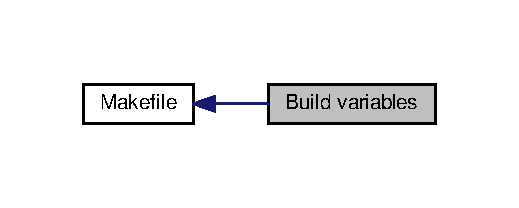
\includegraphics[width=249pt]{group___build___variables}
\end{center}
\end{figure}
\subsection*{Macros}
\begin{DoxyCompactItemize}
\item 
\hypertarget{group___build___variables_ga76ea3cf49247a07c54b3db005a3c7f57}{\#define \hyperlink{group___build___variables_ga76ea3cf49247a07c54b3db005a3c7f57}{C\+O\+N\+F\+I\+G}}\label{group___build___variables_ga76ea3cf49247a07c54b3db005a3c7f57}

\begin{DoxyCompactList}\small\item\em Defines build configuration. Authorized values are 'Release' (by default), 'Debug', or 'Test'. \end{DoxyCompactList}\item 
\hypertarget{group___build___variables_gab6ba1c81d5eb93f6cbcd77db8797b5ad}{\#define \hyperlink{group___build___variables_gab6ba1c81d5eb93f6cbcd77db8797b5ad}{P\+R\+E\+\_\+\+D\+E\+F\+I\+N\+E\+D}}\label{group___build___variables_gab6ba1c81d5eb93f6cbcd77db8797b5ad}

\begin{DoxyCompactList}\small\item\em Stores predefined variables. These variables are passed to the preprocessor. \end{DoxyCompactList}\item 
\hypertarget{group___build___variables_ga4039b19fe99a211262e1b3a58314a4cb}{\#define \hyperlink{group___build___variables_ga4039b19fe99a211262e1b3a58314a4cb}{T\+A\+R\+G\+E\+T\+\_\+\+A\+R\+C\+H}}\label{group___build___variables_ga4039b19fe99a211262e1b3a58314a4cb}

\begin{DoxyCompactList}\small\item\em Defines target architecture. Authorized values are 'x86', 'x86\+\_\+64' (by default), 'arm', 'armhf'. \end{DoxyCompactList}\item 
\hypertarget{group___build___variables_gac49cbbb3d31529b75c2490af64e52695}{\#define \hyperlink{group___build___variables_gac49cbbb3d31529b75c2490af64e52695}{O\+S\+\_\+\+T\+Y\+P\+E}}\label{group___build___variables_gac49cbbb3d31529b75c2490af64e52695}

\begin{DoxyCompactList}\small\item\em Defines target Operating System. Authorized values are 'Linux' (by default), 'Linux64', 'Win32', 'Win64'. \end{DoxyCompactList}\item 
\hypertarget{group___build___variables_ga0811dc6fc274184efa103eab807a0989}{\#define \hyperlink{group___build___variables_ga0811dc6fc274184efa103eab807a0989}{M\+A\+J\+\_\+\+V\+E\+R\+S\+I\+O\+N}}\label{group___build___variables_ga0811dc6fc274184efa103eab807a0989}

\begin{DoxyCompactList}\small\item\em Defines the major version of the binary. The default value is '1'. \end{DoxyCompactList}\item 
\hypertarget{group___build___variables_gabcd45341369f87e7ad5dfefee97c6811}{\#define \hyperlink{group___build___variables_gabcd45341369f87e7ad5dfefee97c6811}{M\+I\+N\+\_\+\+V\+E\+R\+S\+I\+O\+N}}\label{group___build___variables_gabcd45341369f87e7ad5dfefee97c6811}

\begin{DoxyCompactList}\small\item\em Defines the minor version of the binary. The default value is '0'. \end{DoxyCompactList}\item 
\hypertarget{group___build___variables_gad7a967dd260384e94010b31b1412a0b4}{\#define \hyperlink{group___build___variables_gad7a967dd260384e94010b31b1412a0b4}{B\+U\+I\+L\+D\+\_\+\+V\+E\+R\+S\+I\+O\+N}}\label{group___build___variables_gad7a967dd260384e94010b31b1412a0b4}

\begin{DoxyCompactList}\small\item\em Defines the build version of the binary. The default value is '0'. \end{DoxyCompactList}\end{DoxyCompactItemize}


\subsection{Detailed Description}
These variables can be redefined before the execution of 'make'. 


\hypertarget{group___private___variables}{\section{Private\+\_\+\+Variables}
\label{group___private___variables}\index{Private\+\_\+\+Variables@{Private\+\_\+\+Variables}}
}


These variables.  


Collaboration diagram for Private\+\_\+\+Variables\+:
\nopagebreak
\begin{figure}[H]
\begin{center}
\leavevmode
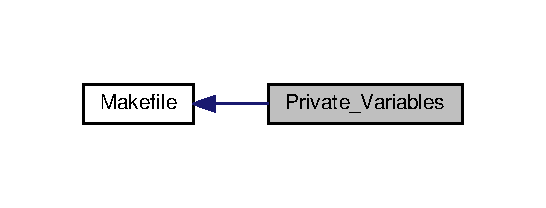
\includegraphics[width=262pt]{group___private___variables}
\end{center}
\end{figure}
\subsection*{Macros}
\begin{DoxyCompactItemize}
\item 
\hypertarget{group___private___variables_ga0a5bb7014615bdedc7fba9605063f8b6}{\#define \hyperlink{group___private___variables_ga0a5bb7014615bdedc7fba9605063f8b6}{R\+E\+V\+\_\+\+N\+U\+M\+B\+E\+R\+\_\+\+F\+I\+L\+E}}\label{group___private___variables_ga0a5bb7014615bdedc7fba9605063f8b6}

\begin{DoxyCompactList}\small\item\em Sets the filename containing the revision number. This filename is 'rev-\/number.\+txt' by default. \end{DoxyCompactList}\item 
\hypertarget{group___private___variables_ga1508c10238d0ce8ebee8aa038ee2869c}{\#define \hyperlink{group___private___variables_ga1508c10238d0ce8ebee8aa038ee2869c}{V\+E\+R\+S\+\_\+\+N\+U\+M\+B\+E\+R\+\_\+\+F\+I\+L\+E}}\label{group___private___variables_ga1508c10238d0ce8ebee8aa038ee2869c}

\begin{DoxyCompactList}\small\item\em Sets the filename containing the version number. This filename is 'vers-\/number.\+txt' by default. It contains the version number in the form x.\+y.\+z where x is the major version, y the minor version and z the build version. \end{DoxyCompactList}\item 
\hypertarget{group___private___variables_gae7e1dc72ef29963f4486a6efe6ad8e04}{\#define \hyperlink{group___private___variables_gae7e1dc72ef29963f4486a6efe6ad8e04}{T\+E\+S\+T\+\_\+\+L\+I\+B}}\label{group___private___variables_gae7e1dc72ef29963f4486a6efe6ad8e04}

\begin{DoxyCompactList}\small\item\em Sets the name of the unit test library. \end{DoxyCompactList}\end{DoxyCompactItemize}


\subsection{Detailed Description}
These variables. 


\hypertarget{group___automatic___variables}{\section{Automatic variables}
\label{group___automatic___variables}\index{Automatic variables@{Automatic variables}}
}


These variables can be redefined during the execution of 'make'.  


Collaboration diagram for Automatic variables\+:
\nopagebreak
\begin{figure}[H]
\begin{center}
\leavevmode
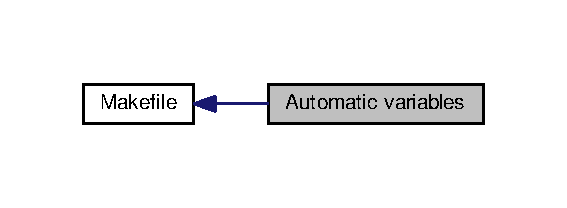
\includegraphics[width=272pt]{group___automatic___variables}
\end{center}
\end{figure}
\subsection*{Macros}
\begin{DoxyCompactItemize}
\item 
\hypertarget{group___automatic___variables_ga1c6d5de492ac61ad29aec7aa9a436bbf}{\#define \hyperlink{group___automatic___variables_ga1c6d5de492ac61ad29aec7aa9a436bbf}{V\+E\+R\+S\+I\+O\+N}}\label{group___automatic___variables_ga1c6d5de492ac61ad29aec7aa9a436bbf}

\begin{DoxyCompactList}\small\item\em Defines the version in the format x.\+y.\+z. \end{DoxyCompactList}\item 
\hypertarget{group___automatic___variables_ga7564a1406feda468ce0cb03cc8f70216}{\#define \hyperlink{group___automatic___variables_ga7564a1406feda468ce0cb03cc8f70216}{B\+I\+N\+A\+R\+Y\+\_\+\+P\+R\+E\+F\+I\+X}}\label{group___automatic___variables_ga7564a1406feda468ce0cb03cc8f70216}

\begin{DoxyCompactList}\small\item\em Sets the prefix of the binary file according to the configuration. \end{DoxyCompactList}\item 
\hypertarget{group___automatic___variables_ga33221a22bc4fd9183788b7a02eb21a1b}{\#define \hyperlink{group___automatic___variables_ga33221a22bc4fd9183788b7a02eb21a1b}{B\+I\+N\+A\+R\+Y\+\_\+\+E\+X\+T}}\label{group___automatic___variables_ga33221a22bc4fd9183788b7a02eb21a1b}

\begin{DoxyCompactList}\small\item\em Sets the extension of the binary file according to the configuration. \end{DoxyCompactList}\item 
\hypertarget{group___automatic___variables_ga15b68a57a767111eeccbb4361ef27d28}{\#define {\bfseries B\+I\+N\+\_\+\+D\+I\+R\+\_\+\+N\+A\+M\+E}}\label{group___automatic___variables_ga15b68a57a767111eeccbb4361ef27d28}

\item 
\hypertarget{group___automatic___variables_gae4c5345f24367773479bbdc89f11ad73}{\#define {\bfseries S\+R\+C\+\_\+\+D\+I\+R\+\_\+\+N\+A\+M\+E}}\label{group___automatic___variables_gae4c5345f24367773479bbdc89f11ad73}

\item 
\hypertarget{group___automatic___variables_ga7824bb533c1132aa392dc850e8cab836}{\#define {\bfseries I\+N\+C\+\_\+\+D\+I\+R\+\_\+\+N\+A\+M\+E}}\label{group___automatic___variables_ga7824bb533c1132aa392dc850e8cab836}

\item 
\hypertarget{group___automatic___variables_ga741001f8715eba92ba3f154de62a16ed}{\#define {\bfseries L\+O\+G\+\_\+\+D\+I\+R\+\_\+\+N\+A\+M\+E}}\label{group___automatic___variables_ga741001f8715eba92ba3f154de62a16ed}

\item 
\hypertarget{group___automatic___variables_gaa7bd71e6a1d9206071565efb4c41d03c}{\#define {\bfseries T\+E\+S\+T\+\_\+\+D\+I\+R\+\_\+\+N\+A\+M\+E}}\label{group___automatic___variables_gaa7bd71e6a1d9206071565efb4c41d03c}

\item 
\hypertarget{group___automatic___variables_ga7812f6263b920beedc05a29cb73bcf8e}{\#define \hyperlink{group___automatic___variables_ga7812f6263b920beedc05a29cb73bcf8e}{P\+R\+O\+J\+E\+C\+T\+\_\+\+D\+I\+R}}\label{group___automatic___variables_ga7812f6263b920beedc05a29cb73bcf8e}

\begin{DoxyCompactList}\small\item\em Reads actual directory corresponding to project name. \end{DoxyCompactList}\item 
\hypertarget{group___automatic___variables_gace0ce5c5385c943349972405f2ada479}{\#define \hyperlink{group___automatic___variables_gace0ce5c5385c943349972405f2ada479}{W\+O\+R\+K\+S\+P\+A\+C\+E\+\_\+\+D\+I\+R}}\label{group___automatic___variables_gace0ce5c5385c943349972405f2ada479}

\begin{DoxyCompactList}\small\item\em Defines Workspace directory. \end{DoxyCompactList}\item 
\hypertarget{group___automatic___variables_ga3160a3fa704cbc54d669767276e0124f}{\#define \hyperlink{group___automatic___variables_ga3160a3fa704cbc54d669767276e0124f}{S\+R\+C\+\_\+\+D\+I\+R}}\label{group___automatic___variables_ga3160a3fa704cbc54d669767276e0124f}

\begin{DoxyCompactList}\small\item\em Defines the parent directory of sources. \end{DoxyCompactList}\item 
\hypertarget{group___automatic___variables_ga310dd0d61daffc990beba1d19af9f47e}{\#define \hyperlink{group___automatic___variables_ga310dd0d61daffc990beba1d19af9f47e}{S\+R\+C\+\_\+\+S\+U\+B\+D\+I\+R}}\label{group___automatic___variables_ga310dd0d61daffc990beba1d19af9f47e}

\begin{DoxyCompactList}\small\item\em Defines the sub-\/directories of sources. \end{DoxyCompactList}\item 
\hypertarget{group___automatic___variables_gaba8cb34a85a8822c9b79de9cfecd4595}{\#define \hyperlink{group___automatic___variables_gaba8cb34a85a8822c9b79de9cfecd4595}{T\+E\+S\+T\+\_\+\+D\+I\+R}}\label{group___automatic___variables_gaba8cb34a85a8822c9b79de9cfecd4595}

\begin{DoxyCompactList}\small\item\em Defines the parent directory of unit testing sources. \end{DoxyCompactList}\item 
\hypertarget{group___automatic___variables_gae17fcd1b9014452d5d23b21e7be729e3}{\#define \hyperlink{group___automatic___variables_gae17fcd1b9014452d5d23b21e7be729e3}{B\+I\+N\+\_\+\+D\+I\+R}}\label{group___automatic___variables_gae17fcd1b9014452d5d23b21e7be729e3}

\begin{DoxyCompactList}\small\item\em Defines the parent directory of binaries. \end{DoxyCompactList}\item 
\hypertarget{group___automatic___variables_ga462faf854129d378edf6f5ae9b649e98}{\#define \hyperlink{group___automatic___variables_ga462faf854129d378edf6f5ae9b649e98}{I\+N\+C\+\_\+\+D\+I\+R}}\label{group___automatic___variables_ga462faf854129d378edf6f5ae9b649e98}

\begin{DoxyCompactList}\small\item\em Defines directory for header files to be deployed with the project binary. \end{DoxyCompactList}\item 
\hypertarget{group___automatic___variables_gaffb9faa4be2c44d33e8a56d4125927bd}{\#define \hyperlink{group___automatic___variables_gaffb9faa4be2c44d33e8a56d4125927bd}{T\+E\+S\+T\+\_\+\+I\+N\+C\+\_\+\+D\+I\+R}}\label{group___automatic___variables_gaffb9faa4be2c44d33e8a56d4125927bd}

\begin{DoxyCompactList}\small\item\em Defines directory for header files required for unit testing. \end{DoxyCompactList}\item 
\hypertarget{group___automatic___variables_ga89fe815a0420a7fda6a4e106263e122b}{\#define \hyperlink{group___automatic___variables_ga89fe815a0420a7fda6a4e106263e122b}{O\+B\+J\+\_\+\+D\+I\+R}}\label{group___automatic___variables_ga89fe815a0420a7fda6a4e106263e122b}

\begin{DoxyCompactList}\small\item\em Defines directory where the object files will be stored during compilation. \end{DoxyCompactList}\item 
\hypertarget{group___automatic___variables_gacd4d3023d24d5314b895981b17825666}{\#define \hyperlink{group___automatic___variables_gacd4d3023d24d5314b895981b17825666}{L\+O\+G\+\_\+\+D\+I\+R}}\label{group___automatic___variables_gacd4d3023d24d5314b895981b17825666}

\begin{DoxyCompactList}\small\item\em Defines directory where the report files will be stored. \end{DoxyCompactList}\item 
\hypertarget{group___automatic___variables_gaeb1e240a5017a152cb83d53ef5b7ab6f}{\#define \hyperlink{group___automatic___variables_gaeb1e240a5017a152cb83d53ef5b7ab6f}{R\+E\+V\+\_\+\+N\+U\+M\+B\+E\+R}}\label{group___automatic___variables_gaeb1e240a5017a152cb83d53ef5b7ab6f}

\begin{DoxyCompactList}\small\item\em Contains the revision number. This number is read from R\+E\+V\+\_\+\+N\+U\+M\+B\+E\+R\+\_\+\+F\+I\+L\+E. \end{DoxyCompactList}\item 
\hypertarget{group___automatic___variables_gac64971050f0b554124e183aa13f22caa}{\#define \hyperlink{group___automatic___variables_gac64971050f0b554124e183aa13f22caa}{C\+\_\+\+S\+O\+U\+R\+C\+E\+S}}\label{group___automatic___variables_gac64971050f0b554124e183aa13f22caa}

\begin{DoxyCompactList}\small\item\em Defines the list of c source files. \end{DoxyCompactList}\item 
\hypertarget{group___automatic___variables_ga8b7fa1d8593b0d2c64abdcfcbda9495b}{\#define \hyperlink{group___automatic___variables_ga8b7fa1d8593b0d2c64abdcfcbda9495b}{C\+X\+X\+\_\+\+S\+O\+U\+R\+C\+E\+S}}\label{group___automatic___variables_ga8b7fa1d8593b0d2c64abdcfcbda9495b}

\begin{DoxyCompactList}\small\item\em Defines the list of c++ source files. \end{DoxyCompactList}\item 
\hypertarget{group___automatic___variables_gafd792eabc9b9a2f7c2a9f193cde29bf6}{\#define \hyperlink{group___automatic___variables_gafd792eabc9b9a2f7c2a9f193cde29bf6}{C\+\_\+\+T\+E\+S\+T\+\_\+\+S\+O\+U\+R\+C\+E\+S}}\label{group___automatic___variables_gafd792eabc9b9a2f7c2a9f193cde29bf6}

\begin{DoxyCompactList}\small\item\em Defines the list of unit tests c source files. \end{DoxyCompactList}\item 
\hypertarget{group___automatic___variables_gabde2d0c19d9087032f2b1d8c16972b1e}{\#define \hyperlink{group___automatic___variables_gabde2d0c19d9087032f2b1d8c16972b1e}{C\+X\+X\+\_\+\+T\+E\+S\+T\+\_\+\+S\+O\+U\+R\+C\+E\+S}}\label{group___automatic___variables_gabde2d0c19d9087032f2b1d8c16972b1e}

\begin{DoxyCompactList}\small\item\em Defines the list of unit tests c++ source files. \end{DoxyCompactList}\item 
\hypertarget{group___automatic___variables_ga0beadd0eb153f706961cebefbb951c45}{\#define \hyperlink{group___automatic___variables_ga0beadd0eb153f706961cebefbb951c45}{S\+O\+U\+R\+C\+E\+S}}\label{group___automatic___variables_ga0beadd0eb153f706961cebefbb951c45}

\begin{DoxyCompactList}\small\item\em Defines the list of c and c++ source files. \end{DoxyCompactList}\item 
\hypertarget{group___automatic___variables_ga4a5f22a280949c97a0cb0d4213275126}{\#define \hyperlink{group___automatic___variables_ga4a5f22a280949c97a0cb0d4213275126}{O\+B\+J\+\_\+\+L\+I\+S\+T}}\label{group___automatic___variables_ga4a5f22a280949c97a0cb0d4213275126}

\begin{DoxyCompactList}\small\item\em Defines the list of object files. \end{DoxyCompactList}\item 
\hypertarget{group___automatic___variables_ga4a067492d681fbbce4157face2f51c27}{\#define \hyperlink{group___automatic___variables_ga4a067492d681fbbce4157face2f51c27}{O\+B\+J\+E\+C\+T\+S}}\label{group___automatic___variables_ga4a067492d681fbbce4157face2f51c27}

\begin{DoxyCompactList}\small\item\em Defines the list of object files. \end{DoxyCompactList}\item 
\hypertarget{group___automatic___variables_ga99aee6cf7d785eaef47006c028971a01}{\#define \hyperlink{group___automatic___variables_ga99aee6cf7d785eaef47006c028971a01}{D\+E\+P\+\_\+\+F\+I\+L\+E\+S}}\label{group___automatic___variables_ga99aee6cf7d785eaef47006c028971a01}

\begin{DoxyCompactList}\small\item\em Establish the list of dependency files from the list of object files. \end{DoxyCompactList}\item 
\hypertarget{group___automatic___variables_ga2a0556694137e2667fb6564e99e2dcef}{\#define \hyperlink{group___automatic___variables_ga2a0556694137e2667fb6564e99e2dcef}{L\+O\+C\+A\+L\+\_\+\+A\+R\+C\+H}}\label{group___automatic___variables_ga2a0556694137e2667fb6564e99e2dcef}

\begin{DoxyCompactList}\small\item\em Stores host architecture. \end{DoxyCompactList}\item 
\#define \hyperlink{group___automatic___variables_ga9682580d83fbc88967858af8593df6df}{A\+R\+M\+\_\+\+F\+A\+M\+I\+L\+Y}
\begin{DoxyCompactList}\small\item\em Stores the A\+R\+M family. \end{DoxyCompactList}\item 
\hypertarget{group___automatic___variables_ga78d126676907aa89a0adbfbef8282585}{\#define \hyperlink{group___automatic___variables_ga78d126676907aa89a0adbfbef8282585}{C\+C}}\label{group___automatic___variables_ga78d126676907aa89a0adbfbef8282585}

\begin{DoxyCompactList}\small\item\em Stores C compilator executable. \end{DoxyCompactList}\item 
\hypertarget{group___automatic___variables_ga015ed04a5a5b8338fca972afb4ad65d8}{\#define \hyperlink{group___automatic___variables_ga015ed04a5a5b8338fca972afb4ad65d8}{C\+X\+X}}\label{group___automatic___variables_ga015ed04a5a5b8338fca972afb4ad65d8}

\begin{DoxyCompactList}\small\item\em Stores C++ compilator executable. \end{DoxyCompactList}\item 
\hypertarget{group___automatic___variables_ga6f98ae7b0908254a0dfd1627e652bebe}{\#define \hyperlink{group___automatic___variables_ga6f98ae7b0908254a0dfd1627e652bebe}{A\+R}}\label{group___automatic___variables_ga6f98ae7b0908254a0dfd1627e652bebe}

\begin{DoxyCompactList}\small\item\em Stores archiver command. \end{DoxyCompactList}\item 
\hypertarget{group___automatic___variables_ga4608958cdf4c8b8ff0a6e301c4c23ae1}{\#define \hyperlink{group___automatic___variables_ga4608958cdf4c8b8ff0a6e301c4c23ae1}{R\+M}}\label{group___automatic___variables_ga4608958cdf4c8b8ff0a6e301c4c23ae1}

\begin{DoxyCompactList}\small\item\em Stores remove command. \end{DoxyCompactList}\item 
\hypertarget{group___automatic___variables_ga247a4a06dc5d02e8acde675caba677ce}{\#define \hyperlink{group___automatic___variables_ga247a4a06dc5d02e8acde675caba677ce}{A\+R\+M\+\_\+\+F\+L\+A\+G\+S}}\label{group___automatic___variables_ga247a4a06dc5d02e8acde675caba677ce}

\begin{DoxyCompactList}\small\item\em Stores specific A\+R\+M flags for compilation and linking. \end{DoxyCompactList}\item 
\hypertarget{group___automatic___variables_gab5862f1ced0d65238672a6829da70788}{\#define \hyperlink{group___automatic___variables_gab5862f1ced0d65238672a6829da70788}{C\+O\+M\+M\+O\+N\+\_\+\+F\+L\+A\+G\+S}}\label{group___automatic___variables_gab5862f1ced0d65238672a6829da70788}

\begin{DoxyCompactList}\small\item\em Defines the C and C++ common flags (compilation and linking) \end{DoxyCompactList}\item 
\hypertarget{group___automatic___variables_ga14f1a6b464d32bb9b01a1357ef6c1dec}{\#define \hyperlink{group___automatic___variables_ga14f1a6b464d32bb9b01a1357ef6c1dec}{C\+O\+M\+P\+I\+L\+\_\+\+F\+L\+A\+G\+S}}\label{group___automatic___variables_ga14f1a6b464d32bb9b01a1357ef6c1dec}

\begin{DoxyCompactList}\small\item\em Defines the C and C++ common compilation flags. \end{DoxyCompactList}\item 
\hypertarget{group___automatic___variables_gad96068ccba4fb10c1ecd2faac6ca9935}{\#define \hyperlink{group___automatic___variables_gad96068ccba4fb10c1ecd2faac6ca9935}{C\+F\+L\+A\+G\+S}}\label{group___automatic___variables_gad96068ccba4fb10c1ecd2faac6ca9935}

\begin{DoxyCompactList}\small\item\em Defines the C compilation flags. \end{DoxyCompactList}\item 
\hypertarget{group___automatic___variables_gafdfbf6a8a87928f2448e0db6d441bd90}{\#define \hyperlink{group___automatic___variables_gafdfbf6a8a87928f2448e0db6d441bd90}{C\+X\+X\+F\+L\+A\+G\+S}}\label{group___automatic___variables_gafdfbf6a8a87928f2448e0db6d441bd90}

\begin{DoxyCompactList}\small\item\em Defines the C++ compilation flags. \end{DoxyCompactList}\item 
\hypertarget{group___automatic___variables_ga2dd4b41234e5a632ac37afce55156d7d}{\#define \hyperlink{group___automatic___variables_ga2dd4b41234e5a632ac37afce55156d7d}{L\+D\+F\+L\+A\+G\+S}}\label{group___automatic___variables_ga2dd4b41234e5a632ac37afce55156d7d}

\begin{DoxyCompactList}\small\item\em Defines the linker flags. \end{DoxyCompactList}\end{DoxyCompactItemize}


\subsection{Detailed Description}
These variables can be redefined during the execution of 'make'. 



\subsection{Macro Definition Documentation}
\hypertarget{group___automatic___variables_ga9682580d83fbc88967858af8593df6df}{\index{Automatic variables@{Automatic variables}!A\+R\+M\+\_\+\+F\+A\+M\+I\+L\+Y@{A\+R\+M\+\_\+\+F\+A\+M\+I\+L\+Y}}
\index{A\+R\+M\+\_\+\+F\+A\+M\+I\+L\+Y@{A\+R\+M\+\_\+\+F\+A\+M\+I\+L\+Y}!Automatic variables@{Automatic variables}}
\subsubsection[{A\+R\+M\+\_\+\+F\+A\+M\+I\+L\+Y}]{\setlength{\rightskip}{0pt plus 5cm}\#define A\+R\+M\+\_\+\+F\+A\+M\+I\+L\+Y}}\label{group___automatic___variables_ga9682580d83fbc88967858af8593df6df}


Stores the A\+R\+M family. 

The main values allowed are \+: cortex-\/a8, cortex-\/a9, ... 

Definition at line 462 of file Makefile.


\chapter{File Documentation}
\hypertarget{_makefile}{\section{Makefile File Reference}
\label{_makefile}\index{Makefile@{Makefile}}
}


Generic project build file.  


\subsection*{Macros}
\begin{DoxyCompactItemize}
\item 
\hypertarget{_makefile_a4b5014034c9aac136ab8c82c2d16dc82}{\#define \hyperlink{_makefile_a4b5014034c9aac136ab8c82c2d16dc82}{C\+O\+L\+O\+R}}\label{_makefile_a4b5014034c9aac136ab8c82c2d16dc82}

\begin{DoxyCompactList}\small\item\em Sets the escape command to display messages in color. \end{DoxyCompactList}\item 
\hypertarget{_makefile_a475df0d9bbf72a496b3b362ef75a2a0f}{\#define \hyperlink{_makefile_a475df0d9bbf72a496b3b362ef75a2a0f}{E\+N\+D\+\_\+\+C\+O\+L\+O\+R}}\label{_makefile_a475df0d9bbf72a496b3b362ef75a2a0f}

\begin{DoxyCompactList}\small\item\em Sets the escape command to complete the colorization. \end{DoxyCompactList}\item 
\hypertarget{group___project___variables_gae73053051efbb45c3a39751f5ce9fb36}{\#define \hyperlink{group___project___variables_gae73053051efbb45c3a39751f5ce9fb36}{P\+R\+O\+J\+E\+C\+T\+\_\+\+N\+A\+M\+E}}\label{group___project___variables_gae73053051efbb45c3a39751f5ce9fb36}

\begin{DoxyCompactList}\small\item\em Defines the project name. This name must match the name of the project's parent directory in the workspace. \end{DoxyCompactList}\item 
\hypertarget{group___project___variables_gad661cebbb68b497f00fba5676c36eaea}{\#define \hyperlink{group___project___variables_gad661cebbb68b497f00fba5676c36eaea}{D\+E\+P\+E\+N\+D\+E\+N\+C\+I\+E\+S}}\label{group___project___variables_gad661cebbb68b497f00fba5676c36eaea}

\begin{DoxyCompactList}\small\item\em Sets the name of libraries whose binary depends. These libraries must be in a path of the L\+D\+\_\+\+L\+I\+B\+R\+A\+R\+Y\+\_\+\+P\+A\+T\+H variable, in the system default directories, or in workspace. \end{DoxyCompactList}\item 
\hypertarget{group___project___variables_ga36eaa1244b8f912226a6211c0300afd1}{\#define \hyperlink{group___project___variables_ga36eaa1244b8f912226a6211c0300afd1}{T\+E\+S\+T\+\_\+\+D\+E\+P\+E\+N\+D\+E\+N\+C\+I\+E\+S}}\label{group___project___variables_ga36eaa1244b8f912226a6211c0300afd1}

\begin{DoxyCompactList}\small\item\em Sets the name of libraries whose unit testing depends. These libraries must be in a path of the L\+D\+\_\+\+L\+I\+B\+R\+A\+R\+Y\+\_\+\+P\+A\+T\+H variable, in the system default directories, or in workspace. \end{DoxyCompactList}\item 
\hypertarget{group___project___variables_ga84125bd283e4810d75a8be644b522672}{\#define \hyperlink{group___project___variables_ga84125bd283e4810d75a8be644b522672}{L\+I\+B\+\_\+\+D\+I\+R}}\label{group___project___variables_ga84125bd283e4810d75a8be644b522672}

\begin{DoxyCompactList}\small\item\em Defines directory of system libraries. This variable can be set before calling 'make'. \end{DoxyCompactList}\item 
\hypertarget{group___project___variables_gaff7229fc1fa8b5497265124671da29b2}{\#define \hyperlink{group___project___variables_gaff7229fc1fa8b5497265124671da29b2}{T\+E\+S\+T\+\_\+\+L\+I\+B\+\_\+\+D\+I\+R}}\label{group___project___variables_gaff7229fc1fa8b5497265124671da29b2}

\begin{DoxyCompactList}\small\item\em Defines the library directory required for unit testing. This variable can be set before calling 'make'. \end{DoxyCompactList}\item 
\hypertarget{group___project___variables_ga4784add1b0803628960f83525dadc73b}{\#define \hyperlink{group___project___variables_ga4784add1b0803628960f83525dadc73b}{B\+I\+N\+A\+R\+Y\+\_\+\+T\+Y\+P\+E}}\label{group___project___variables_ga4784add1b0803628960f83525dadc73b}

\begin{DoxyCompactList}\small\item\em Defines the type of binary generated. Authorized values are 'exe' (by default), 'lib', or 'shared'. \end{DoxyCompactList}\item 
\hypertarget{group___build___variables_ga76ea3cf49247a07c54b3db005a3c7f57}{\#define \hyperlink{group___build___variables_ga76ea3cf49247a07c54b3db005a3c7f57}{C\+O\+N\+F\+I\+G}}\label{group___build___variables_ga76ea3cf49247a07c54b3db005a3c7f57}

\begin{DoxyCompactList}\small\item\em Defines build configuration. Authorized values are 'Release' (by default), 'Debug', or 'Test'. \end{DoxyCompactList}\item 
\hypertarget{group___build___variables_gab6ba1c81d5eb93f6cbcd77db8797b5ad}{\#define \hyperlink{group___build___variables_gab6ba1c81d5eb93f6cbcd77db8797b5ad}{P\+R\+E\+\_\+\+D\+E\+F\+I\+N\+E\+D}}\label{group___build___variables_gab6ba1c81d5eb93f6cbcd77db8797b5ad}

\begin{DoxyCompactList}\small\item\em Stores predefined variables. These variables are passed to the preprocessor. \end{DoxyCompactList}\item 
\hypertarget{group___build___variables_ga4039b19fe99a211262e1b3a58314a4cb}{\#define \hyperlink{group___build___variables_ga4039b19fe99a211262e1b3a58314a4cb}{T\+A\+R\+G\+E\+T\+\_\+\+A\+R\+C\+H}}\label{group___build___variables_ga4039b19fe99a211262e1b3a58314a4cb}

\begin{DoxyCompactList}\small\item\em Defines target architecture. Authorized values are 'x86', 'x86\+\_\+64' (by default), 'arm', 'armhf'. \end{DoxyCompactList}\item 
\hypertarget{group___build___variables_gac49cbbb3d31529b75c2490af64e52695}{\#define \hyperlink{group___build___variables_gac49cbbb3d31529b75c2490af64e52695}{O\+S\+\_\+\+T\+Y\+P\+E}}\label{group___build___variables_gac49cbbb3d31529b75c2490af64e52695}

\begin{DoxyCompactList}\small\item\em Defines target Operating System. Authorized values are 'Linux' (by default), 'Linux64', 'Win32', 'Win64'. \end{DoxyCompactList}\item 
\hypertarget{group___build___variables_ga0811dc6fc274184efa103eab807a0989}{\#define \hyperlink{group___build___variables_ga0811dc6fc274184efa103eab807a0989}{M\+A\+J\+\_\+\+V\+E\+R\+S\+I\+O\+N}}\label{group___build___variables_ga0811dc6fc274184efa103eab807a0989}

\begin{DoxyCompactList}\small\item\em Defines the major version of the binary. The default value is '1'. \end{DoxyCompactList}\item 
\hypertarget{group___build___variables_gabcd45341369f87e7ad5dfefee97c6811}{\#define \hyperlink{group___build___variables_gabcd45341369f87e7ad5dfefee97c6811}{M\+I\+N\+\_\+\+V\+E\+R\+S\+I\+O\+N}}\label{group___build___variables_gabcd45341369f87e7ad5dfefee97c6811}

\begin{DoxyCompactList}\small\item\em Defines the minor version of the binary. The default value is '0'. \end{DoxyCompactList}\item 
\hypertarget{group___build___variables_gad7a967dd260384e94010b31b1412a0b4}{\#define \hyperlink{group___build___variables_gad7a967dd260384e94010b31b1412a0b4}{B\+U\+I\+L\+D\+\_\+\+V\+E\+R\+S\+I\+O\+N}}\label{group___build___variables_gad7a967dd260384e94010b31b1412a0b4}

\begin{DoxyCompactList}\small\item\em Defines the build version of the binary. The default value is '0'. \end{DoxyCompactList}\item 
\hypertarget{group___private___variables_ga0a5bb7014615bdedc7fba9605063f8b6}{\#define \hyperlink{group___private___variables_ga0a5bb7014615bdedc7fba9605063f8b6}{R\+E\+V\+\_\+\+N\+U\+M\+B\+E\+R\+\_\+\+F\+I\+L\+E}}\label{group___private___variables_ga0a5bb7014615bdedc7fba9605063f8b6}

\begin{DoxyCompactList}\small\item\em Sets the filename containing the revision number. This filename is 'rev-\/number.\+txt' by default. \end{DoxyCompactList}\item 
\hypertarget{group___private___variables_ga1508c10238d0ce8ebee8aa038ee2869c}{\#define \hyperlink{group___private___variables_ga1508c10238d0ce8ebee8aa038ee2869c}{V\+E\+R\+S\+\_\+\+N\+U\+M\+B\+E\+R\+\_\+\+F\+I\+L\+E}}\label{group___private___variables_ga1508c10238d0ce8ebee8aa038ee2869c}

\begin{DoxyCompactList}\small\item\em Sets the filename containing the version number. This filename is 'vers-\/number.\+txt' by default. It contains the version number in the form x.\+y.\+z where x is the major version, y the minor version and z the build version. \end{DoxyCompactList}\item 
\hypertarget{group___private___variables_gae7e1dc72ef29963f4486a6efe6ad8e04}{\#define \hyperlink{group___private___variables_gae7e1dc72ef29963f4486a6efe6ad8e04}{T\+E\+S\+T\+\_\+\+L\+I\+B}}\label{group___private___variables_gae7e1dc72ef29963f4486a6efe6ad8e04}

\begin{DoxyCompactList}\small\item\em Sets the name of the unit test library. \end{DoxyCompactList}\item 
\hypertarget{group___automatic___variables_ga1c6d5de492ac61ad29aec7aa9a436bbf}{\#define \hyperlink{group___automatic___variables_ga1c6d5de492ac61ad29aec7aa9a436bbf}{V\+E\+R\+S\+I\+O\+N}}\label{group___automatic___variables_ga1c6d5de492ac61ad29aec7aa9a436bbf}

\begin{DoxyCompactList}\small\item\em Defines the version in the format x.\+y.\+z. \end{DoxyCompactList}\item 
\hypertarget{group___automatic___variables_ga7564a1406feda468ce0cb03cc8f70216}{\#define \hyperlink{group___automatic___variables_ga7564a1406feda468ce0cb03cc8f70216}{B\+I\+N\+A\+R\+Y\+\_\+\+P\+R\+E\+F\+I\+X}}\label{group___automatic___variables_ga7564a1406feda468ce0cb03cc8f70216}

\begin{DoxyCompactList}\small\item\em Sets the prefix of the binary file according to the configuration. \end{DoxyCompactList}\item 
\hypertarget{group___automatic___variables_ga33221a22bc4fd9183788b7a02eb21a1b}{\#define \hyperlink{group___automatic___variables_ga33221a22bc4fd9183788b7a02eb21a1b}{B\+I\+N\+A\+R\+Y\+\_\+\+E\+X\+T}}\label{group___automatic___variables_ga33221a22bc4fd9183788b7a02eb21a1b}

\begin{DoxyCompactList}\small\item\em Sets the extension of the binary file according to the configuration. \end{DoxyCompactList}\item 
\hypertarget{group___automatic___variables_ga15b68a57a767111eeccbb4361ef27d28}{\#define {\bfseries B\+I\+N\+\_\+\+D\+I\+R\+\_\+\+N\+A\+M\+E}}\label{group___automatic___variables_ga15b68a57a767111eeccbb4361ef27d28}

\item 
\hypertarget{group___automatic___variables_gae4c5345f24367773479bbdc89f11ad73}{\#define {\bfseries S\+R\+C\+\_\+\+D\+I\+R\+\_\+\+N\+A\+M\+E}}\label{group___automatic___variables_gae4c5345f24367773479bbdc89f11ad73}

\item 
\hypertarget{group___automatic___variables_ga7824bb533c1132aa392dc850e8cab836}{\#define {\bfseries I\+N\+C\+\_\+\+D\+I\+R\+\_\+\+N\+A\+M\+E}}\label{group___automatic___variables_ga7824bb533c1132aa392dc850e8cab836}

\item 
\hypertarget{group___automatic___variables_ga741001f8715eba92ba3f154de62a16ed}{\#define {\bfseries L\+O\+G\+\_\+\+D\+I\+R\+\_\+\+N\+A\+M\+E}}\label{group___automatic___variables_ga741001f8715eba92ba3f154de62a16ed}

\item 
\hypertarget{group___automatic___variables_gaa7bd71e6a1d9206071565efb4c41d03c}{\#define {\bfseries T\+E\+S\+T\+\_\+\+D\+I\+R\+\_\+\+N\+A\+M\+E}}\label{group___automatic___variables_gaa7bd71e6a1d9206071565efb4c41d03c}

\item 
\hypertarget{group___automatic___variables_ga7812f6263b920beedc05a29cb73bcf8e}{\#define \hyperlink{group___automatic___variables_ga7812f6263b920beedc05a29cb73bcf8e}{P\+R\+O\+J\+E\+C\+T\+\_\+\+D\+I\+R}}\label{group___automatic___variables_ga7812f6263b920beedc05a29cb73bcf8e}

\begin{DoxyCompactList}\small\item\em Reads actual directory corresponding to project name. \end{DoxyCompactList}\item 
\hypertarget{group___automatic___variables_gace0ce5c5385c943349972405f2ada479}{\#define \hyperlink{group___automatic___variables_gace0ce5c5385c943349972405f2ada479}{W\+O\+R\+K\+S\+P\+A\+C\+E\+\_\+\+D\+I\+R}}\label{group___automatic___variables_gace0ce5c5385c943349972405f2ada479}

\begin{DoxyCompactList}\small\item\em Defines Workspace directory. \end{DoxyCompactList}\item 
\hypertarget{group___automatic___variables_ga3160a3fa704cbc54d669767276e0124f}{\#define \hyperlink{group___automatic___variables_ga3160a3fa704cbc54d669767276e0124f}{S\+R\+C\+\_\+\+D\+I\+R}}\label{group___automatic___variables_ga3160a3fa704cbc54d669767276e0124f}

\begin{DoxyCompactList}\small\item\em Defines the parent directory of sources. \end{DoxyCompactList}\item 
\hypertarget{group___automatic___variables_ga310dd0d61daffc990beba1d19af9f47e}{\#define \hyperlink{group___automatic___variables_ga310dd0d61daffc990beba1d19af9f47e}{S\+R\+C\+\_\+\+S\+U\+B\+D\+I\+R}}\label{group___automatic___variables_ga310dd0d61daffc990beba1d19af9f47e}

\begin{DoxyCompactList}\small\item\em Defines the sub-\/directories of sources. \end{DoxyCompactList}\item 
\hypertarget{group___automatic___variables_gaba8cb34a85a8822c9b79de9cfecd4595}{\#define \hyperlink{group___automatic___variables_gaba8cb34a85a8822c9b79de9cfecd4595}{T\+E\+S\+T\+\_\+\+D\+I\+R}}\label{group___automatic___variables_gaba8cb34a85a8822c9b79de9cfecd4595}

\begin{DoxyCompactList}\small\item\em Defines the parent directory of unit testing sources. \end{DoxyCompactList}\item 
\hypertarget{group___automatic___variables_gae17fcd1b9014452d5d23b21e7be729e3}{\#define \hyperlink{group___automatic___variables_gae17fcd1b9014452d5d23b21e7be729e3}{B\+I\+N\+\_\+\+D\+I\+R}}\label{group___automatic___variables_gae17fcd1b9014452d5d23b21e7be729e3}

\begin{DoxyCompactList}\small\item\em Defines the parent directory of binaries. \end{DoxyCompactList}\item 
\hypertarget{group___automatic___variables_ga462faf854129d378edf6f5ae9b649e98}{\#define \hyperlink{group___automatic___variables_ga462faf854129d378edf6f5ae9b649e98}{I\+N\+C\+\_\+\+D\+I\+R}}\label{group___automatic___variables_ga462faf854129d378edf6f5ae9b649e98}

\begin{DoxyCompactList}\small\item\em Defines directory for header files to be deployed with the project binary. \end{DoxyCompactList}\item 
\hypertarget{group___automatic___variables_gaffb9faa4be2c44d33e8a56d4125927bd}{\#define \hyperlink{group___automatic___variables_gaffb9faa4be2c44d33e8a56d4125927bd}{T\+E\+S\+T\+\_\+\+I\+N\+C\+\_\+\+D\+I\+R}}\label{group___automatic___variables_gaffb9faa4be2c44d33e8a56d4125927bd}

\begin{DoxyCompactList}\small\item\em Defines directory for header files required for unit testing. \end{DoxyCompactList}\item 
\hypertarget{group___automatic___variables_ga89fe815a0420a7fda6a4e106263e122b}{\#define \hyperlink{group___automatic___variables_ga89fe815a0420a7fda6a4e106263e122b}{O\+B\+J\+\_\+\+D\+I\+R}}\label{group___automatic___variables_ga89fe815a0420a7fda6a4e106263e122b}

\begin{DoxyCompactList}\small\item\em Defines directory where the object files will be stored during compilation. \end{DoxyCompactList}\item 
\hypertarget{group___automatic___variables_gacd4d3023d24d5314b895981b17825666}{\#define \hyperlink{group___automatic___variables_gacd4d3023d24d5314b895981b17825666}{L\+O\+G\+\_\+\+D\+I\+R}}\label{group___automatic___variables_gacd4d3023d24d5314b895981b17825666}

\begin{DoxyCompactList}\small\item\em Defines directory where the report files will be stored. \end{DoxyCompactList}\item 
\hypertarget{group___automatic___variables_gaeb1e240a5017a152cb83d53ef5b7ab6f}{\#define \hyperlink{group___automatic___variables_gaeb1e240a5017a152cb83d53ef5b7ab6f}{R\+E\+V\+\_\+\+N\+U\+M\+B\+E\+R}}\label{group___automatic___variables_gaeb1e240a5017a152cb83d53ef5b7ab6f}

\begin{DoxyCompactList}\small\item\em Contains the revision number. This number is read from R\+E\+V\+\_\+\+N\+U\+M\+B\+E\+R\+\_\+\+F\+I\+L\+E. \end{DoxyCompactList}\item 
\hypertarget{group___automatic___variables_gac64971050f0b554124e183aa13f22caa}{\#define \hyperlink{group___automatic___variables_gac64971050f0b554124e183aa13f22caa}{C\+\_\+\+S\+O\+U\+R\+C\+E\+S}}\label{group___automatic___variables_gac64971050f0b554124e183aa13f22caa}

\begin{DoxyCompactList}\small\item\em Defines the list of c source files. \end{DoxyCompactList}\item 
\hypertarget{group___automatic___variables_ga8b7fa1d8593b0d2c64abdcfcbda9495b}{\#define \hyperlink{group___automatic___variables_ga8b7fa1d8593b0d2c64abdcfcbda9495b}{C\+X\+X\+\_\+\+S\+O\+U\+R\+C\+E\+S}}\label{group___automatic___variables_ga8b7fa1d8593b0d2c64abdcfcbda9495b}

\begin{DoxyCompactList}\small\item\em Defines the list of c++ source files. \end{DoxyCompactList}\item 
\hypertarget{group___automatic___variables_gafd792eabc9b9a2f7c2a9f193cde29bf6}{\#define \hyperlink{group___automatic___variables_gafd792eabc9b9a2f7c2a9f193cde29bf6}{C\+\_\+\+T\+E\+S\+T\+\_\+\+S\+O\+U\+R\+C\+E\+S}}\label{group___automatic___variables_gafd792eabc9b9a2f7c2a9f193cde29bf6}

\begin{DoxyCompactList}\small\item\em Defines the list of unit tests c source files. \end{DoxyCompactList}\item 
\hypertarget{group___automatic___variables_gabde2d0c19d9087032f2b1d8c16972b1e}{\#define \hyperlink{group___automatic___variables_gabde2d0c19d9087032f2b1d8c16972b1e}{C\+X\+X\+\_\+\+T\+E\+S\+T\+\_\+\+S\+O\+U\+R\+C\+E\+S}}\label{group___automatic___variables_gabde2d0c19d9087032f2b1d8c16972b1e}

\begin{DoxyCompactList}\small\item\em Defines the list of unit tests c++ source files. \end{DoxyCompactList}\item 
\hypertarget{group___automatic___variables_ga0beadd0eb153f706961cebefbb951c45}{\#define \hyperlink{group___automatic___variables_ga0beadd0eb153f706961cebefbb951c45}{S\+O\+U\+R\+C\+E\+S}}\label{group___automatic___variables_ga0beadd0eb153f706961cebefbb951c45}

\begin{DoxyCompactList}\small\item\em Defines the list of c and c++ source files. \end{DoxyCompactList}\item 
\hypertarget{group___automatic___variables_ga4a5f22a280949c97a0cb0d4213275126}{\#define \hyperlink{group___automatic___variables_ga4a5f22a280949c97a0cb0d4213275126}{O\+B\+J\+\_\+\+L\+I\+S\+T}}\label{group___automatic___variables_ga4a5f22a280949c97a0cb0d4213275126}

\begin{DoxyCompactList}\small\item\em Defines the list of object files. \end{DoxyCompactList}\item 
\hypertarget{group___automatic___variables_ga4a067492d681fbbce4157face2f51c27}{\#define \hyperlink{group___automatic___variables_ga4a067492d681fbbce4157face2f51c27}{O\+B\+J\+E\+C\+T\+S}}\label{group___automatic___variables_ga4a067492d681fbbce4157face2f51c27}

\begin{DoxyCompactList}\small\item\em Defines the list of object files. \end{DoxyCompactList}\item 
\hypertarget{group___automatic___variables_ga99aee6cf7d785eaef47006c028971a01}{\#define \hyperlink{group___automatic___variables_ga99aee6cf7d785eaef47006c028971a01}{D\+E\+P\+\_\+\+F\+I\+L\+E\+S}}\label{group___automatic___variables_ga99aee6cf7d785eaef47006c028971a01}

\begin{DoxyCompactList}\small\item\em Establish the list of dependency files from the list of object files. \end{DoxyCompactList}\item 
\hypertarget{group___automatic___variables_ga2a0556694137e2667fb6564e99e2dcef}{\#define \hyperlink{group___automatic___variables_ga2a0556694137e2667fb6564e99e2dcef}{L\+O\+C\+A\+L\+\_\+\+A\+R\+C\+H}}\label{group___automatic___variables_ga2a0556694137e2667fb6564e99e2dcef}

\begin{DoxyCompactList}\small\item\em Stores host architecture. \end{DoxyCompactList}\item 
\#define \hyperlink{group___automatic___variables_ga9682580d83fbc88967858af8593df6df}{A\+R\+M\+\_\+\+F\+A\+M\+I\+L\+Y}
\begin{DoxyCompactList}\small\item\em Stores the A\+R\+M family. \end{DoxyCompactList}\item 
\hypertarget{group___automatic___variables_ga78d126676907aa89a0adbfbef8282585}{\#define \hyperlink{group___automatic___variables_ga78d126676907aa89a0adbfbef8282585}{C\+C}}\label{group___automatic___variables_ga78d126676907aa89a0adbfbef8282585}

\begin{DoxyCompactList}\small\item\em Stores C compilator executable. \end{DoxyCompactList}\item 
\hypertarget{group___automatic___variables_ga015ed04a5a5b8338fca972afb4ad65d8}{\#define \hyperlink{group___automatic___variables_ga015ed04a5a5b8338fca972afb4ad65d8}{C\+X\+X}}\label{group___automatic___variables_ga015ed04a5a5b8338fca972afb4ad65d8}

\begin{DoxyCompactList}\small\item\em Stores C++ compilator executable. \end{DoxyCompactList}\item 
\hypertarget{group___automatic___variables_ga6f98ae7b0908254a0dfd1627e652bebe}{\#define \hyperlink{group___automatic___variables_ga6f98ae7b0908254a0dfd1627e652bebe}{A\+R}}\label{group___automatic___variables_ga6f98ae7b0908254a0dfd1627e652bebe}

\begin{DoxyCompactList}\small\item\em Stores archiver command. \end{DoxyCompactList}\item 
\hypertarget{group___automatic___variables_ga4608958cdf4c8b8ff0a6e301c4c23ae1}{\#define \hyperlink{group___automatic___variables_ga4608958cdf4c8b8ff0a6e301c4c23ae1}{R\+M}}\label{group___automatic___variables_ga4608958cdf4c8b8ff0a6e301c4c23ae1}

\begin{DoxyCompactList}\small\item\em Stores remove command. \end{DoxyCompactList}\item 
\hypertarget{group___automatic___variables_ga247a4a06dc5d02e8acde675caba677ce}{\#define \hyperlink{group___automatic___variables_ga247a4a06dc5d02e8acde675caba677ce}{A\+R\+M\+\_\+\+F\+L\+A\+G\+S}}\label{group___automatic___variables_ga247a4a06dc5d02e8acde675caba677ce}

\begin{DoxyCompactList}\small\item\em Stores specific A\+R\+M flags for compilation and linking. \end{DoxyCompactList}\item 
\hypertarget{group___automatic___variables_gab5862f1ced0d65238672a6829da70788}{\#define \hyperlink{group___automatic___variables_gab5862f1ced0d65238672a6829da70788}{C\+O\+M\+M\+O\+N\+\_\+\+F\+L\+A\+G\+S}}\label{group___automatic___variables_gab5862f1ced0d65238672a6829da70788}

\begin{DoxyCompactList}\small\item\em Defines the C and C++ common flags (compilation and linking) \end{DoxyCompactList}\item 
\hypertarget{group___automatic___variables_ga14f1a6b464d32bb9b01a1357ef6c1dec}{\#define \hyperlink{group___automatic___variables_ga14f1a6b464d32bb9b01a1357ef6c1dec}{C\+O\+M\+P\+I\+L\+\_\+\+F\+L\+A\+G\+S}}\label{group___automatic___variables_ga14f1a6b464d32bb9b01a1357ef6c1dec}

\begin{DoxyCompactList}\small\item\em Defines the C and C++ common compilation flags. \end{DoxyCompactList}\item 
\hypertarget{group___automatic___variables_gad96068ccba4fb10c1ecd2faac6ca9935}{\#define \hyperlink{group___automatic___variables_gad96068ccba4fb10c1ecd2faac6ca9935}{C\+F\+L\+A\+G\+S}}\label{group___automatic___variables_gad96068ccba4fb10c1ecd2faac6ca9935}

\begin{DoxyCompactList}\small\item\em Defines the C compilation flags. \end{DoxyCompactList}\item 
\hypertarget{group___automatic___variables_gafdfbf6a8a87928f2448e0db6d441bd90}{\#define \hyperlink{group___automatic___variables_gafdfbf6a8a87928f2448e0db6d441bd90}{C\+X\+X\+F\+L\+A\+G\+S}}\label{group___automatic___variables_gafdfbf6a8a87928f2448e0db6d441bd90}

\begin{DoxyCompactList}\small\item\em Defines the C++ compilation flags. \end{DoxyCompactList}\item 
\hypertarget{group___automatic___variables_ga2dd4b41234e5a632ac37afce55156d7d}{\#define \hyperlink{group___automatic___variables_ga2dd4b41234e5a632ac37afce55156d7d}{L\+D\+F\+L\+A\+G\+S}}\label{group___automatic___variables_ga2dd4b41234e5a632ac37afce55156d7d}

\begin{DoxyCompactList}\small\item\em Defines the linker flags. \end{DoxyCompactList}\end{DoxyCompactItemize}


\subsection{Detailed Description}
Generic project build file. 



 

 $\ast$$\ast$ Copyright (c) 2018 by Tuxin $\ast$$\ast$ $\ast$$\ast$ All Rights Reserved $\ast$$\ast$ 

 $\ast$$\ast$ Version 1.\+0.\+0 April 25, 2018 $\ast$$\ast$ 

 

 

 \begin{DoxyVerb}         This makefile can generate a binary by automatically detecting
         the files of a project, provided that it respects a pre-defined
         directory architecture.
\end{DoxyVerb}


\begin{DoxyAuthor}{Author}
Tuxin (Jean-\/\+Pierre) 
\end{DoxyAuthor}
\begin{DoxyVersion}{Version}
1.\+0.\+0 
\end{DoxyVersion}
\begin{DoxySince}{Since}
Created 04/25/2018 (J\+P\+B) 
\end{DoxySince}
\begin{DoxyDate}{Date}
April 25, 2018
\end{DoxyDate}




Definition in file \hyperlink{_makefile_source}{Makefile}.


%--- End generated contents ---

% Index
\newpage
\phantomsection
\addcontentsline{toc}{chapter}{Index}
\printindex

\end{document}
